\documentclass[a4paper,12pt]{article} % тип документа

% Поля страниц
\usepackage[left=2.5cm,right=2.5cm,
    top=2cm,bottom=2cm,bindingoffset=0cm]{geometry}
    
%Пакет дял таблиц   
\usepackage{multirow} 
    
%Отступ после заголовка    
\usepackage{indentfirst}


% Рисунки
\usepackage{floatrow,graphicx,calc}
\usepackage{wrapfig}

%%% Работа с картинками
\usepackage{graphicx}  % Для вставки рисунков
\graphicspath{{images/}{images2/}}  % папки с картинками
\setlength\fboxsep{3pt} % Отступ рамки \fbox{} от рисунка
\setlength\fboxrule{1pt} % Толщина линий рамки \fbox{}
\usepackage{wrapfig} % Обтекание рисунков и таблиц текстом

% Создаёем новый разделитель
\DeclareFloatSeparators{mysep}{\hspace{1cm}}

% Ссылки?
\usepackage{hyperref}
\usepackage[rgb]{xcolor}
\hypersetup{				% Гиперссылки
    colorlinks=true,       	% false: ссылки в рамках
	urlcolor=blue          % на URL
}


%  Русский язык
\usepackage[T2A]{fontenc}			% кодировка
\usepackage[utf8]{inputenc}			% кодировка исходного текста
\usepackage[english,russian]{babel}	% локализация и переносы




% Математика
\usepackage{amsmath,amsfonts,amssymb,amsthm,mathtools}

%%% Дополнительная работа с математикой
\usepackage{amsmath,amsfonts,amssymb,amsthm,mathtools} % AMS
\usepackage{icomma} % "Умная" запятая: $0,2$ --- число, $0, 2$ --- перечисление


% Что-то 
\usepackage{wasysym}


\begin{document}
\begin{center}
	\footnotesize{МОСКОВСКИЙ ФИЗИКО-ТЕХНИЧЕСКИЙ ИНСТИТУТ\\(НАЦИОНАЛЬНЫЙ 			ИССЛЕДОВАТЕЛЬСКИЙ УНИВЕРСИТЕТ)}\\
	\footnotesize{ФИЗТЕХ-ШКОЛА РАДИОТЕХНИКИ И КОМПЬЮТЕРНЫХ ТЕХНОЛОГИЙ\\}
	\hfill \break
	\hfill \break
	\hfill \break
	\hfill \break
	\hfill \break
	\hfill \break
\end{center}

\begin{center}   
    \hfill \break
	\hfill \break
	\hfill \break
	\hfill \break
	\hfill \break
	\hfill \break
	\hfill \break
	\hfill \break
	\hfill \break
	\hfill \break
	\hfill \break
	\large{Вопрос по выбору, 3 семестр\\\large{\textbf{Закон Кюри-Вейсса}}}\\
	\hfill \break
	\hfill \break
	\hfill \break
	\hfill \break
	\hfill \break
	\hfill \break
	\hfill \break
	\hfill \break
	\hfill \break
	\hfill \break
	\hfill \break
	\begin{flushright}
		Климова Екатерина\\
		Группа Б01-108
	\end{flushright}
	\hfill \break
\end{center}
\hfill \break
\hfill \break
\begin{center}
	Долгопрудный, 2022 г.
\end{center}
\thispagestyle{empty}

\newpage
\hfill \break
\textbf{Цель работы:} изучение температурной зависимости магнитной восприимчивости ферромагнетика выше точки Кюри.
\hfill \break
\hfill \break
\textbf{В работе используются:} катушка самоиндукции с образцом из гадолиния; термостат; частотомер; цифровой вольтметр; $LC$-автогенератор; термопара медь-константан.

\section{Аннотация}
\hfill \break В данной работе проводится исследование зависимости периода колебаний автогенератора от температуры сердечника катушки и по результатам измерений определяется парамагнитная точка Кюри гадолиния.

\section{Теоретическое введение}
\subsection{Магнитное поле в веществе}
\hfill \break В веществе магнитное поле формируется как внешним полем, так и циркулирующими в этом веществе токами. На микроуровне (то есть на расстояниях порядка размера атома и менее) поле резко меняется во времени и пространстве. Это поле называется микрополем $\textbf{B}_\text{микро}$. Однако если произвести усреднение по малому объему $\Delta V$, в котором, тем не менее, имеется много частиц зарядов, то получим среднее поле: $\textbf{B} = \frac{1}{\Delta V} \int_{\Delta V} \textbf{B}_\text{микро} \,dV$. Среднее поле меняется существенно медленнее вследствие статистического усреднения при случайном движении частиц. Вектор $\textbf{B}$ называют \textit{индукцией} магнитного поля.

\hfill \break При макроскопическом описании свойств среды можно считать, что каждый элемент объема среды может являться элементарным источником магнитного поля $-$ магнитным диполем. Для описания усредненных свойств среды используют \textit{вектор намагниченности} $\textbf{M}$, равный магнитному моменту единичного объема вещества.

\hfill \break Также вводится вектор \textit{напряженности} магнитного поля $\textbf{H}$, удовлетворяющий соотношению (в СГСЭ):

\begin{equation}\label{ linkname }
\textbf{B} = \textbf{H}+4\pi \textbf{M}.
\end{equation}

\hfill \break В наиболее простом случае намагниченность в каждой точке среды прямо пропорциональна вектору напряженности в этой же точке:

\begin{equation}\label{ linkname }
\textbf{M} = \chi \textbf{H},
\end{equation}

\hfill \break где $\chi$ $-$ \textit{магнитная восприимчивость}, в зависимости от значения которой можно условно выделить два типа веществ: \textit{диамагнетики} ($\chi < 0$), в которых элементарные диполи ориентированы в основном против приложенного поля, и \textit{парамагнетики} ($\chi > 0$), в которых элементарные диполи ориентированы в основном по направлению приложенного поля. В общем случае зависимость $\textbf{M}(\textbf{H})$ не является линейной, а зависит от предыстории образца $-$ явление гистерезиса в \textit{ферромагнетиках}.

\hfill \break Если закон (2) применим, то

\begin{equation}\label{ linkname }
\textbf{B} = \mu \textbf{H},
\end{equation}

\hfill \break где $\mu = 1 + 4\pi\chi$ $-$ \textit{магнитная проницаемость} вещества.

\subsection{Парамагнетизм}
\hfill \break Парамагнетизм наблюдается у тех веществ, атомы которых обладают магнитными моментами уже в отсутствие внешнего магнитного поля. В парамагнетиках энергия взаимодействия между соседними магнитными моментами атомов мала по сравнению с тепловой энергией, поэтому пока нет магнитного поля, атомы совершают беспорядочное тепловое движение, а их магнитные моменты ориентированы в пространстве также беспорядочно. В этом случае вещество не намагничено. При помещении во внешнее поле магнитным моментам энергетически выгодно ориентироваться преимущественно по полю, что и приводит к парамагнитному эффекту: $\chi > 0$, то есть $\textbf{B} || \textbf{H} || \textbf{M}$. 

\hfill \break Оценим зависимость магнитной восприимчивости парамагнетика от температуры. Пусть среднее число атомов в единице объема равно $n$, а величина магнитного момента атома $-$ $p_{m}$. В магнитном поле с индукцией $B$ энергия магнитного диполя, составляющего с направлением поля угол $\alpha$, равна

$$
|U| = p_{m}B\cos{\alpha}
$$

\hfill \break и может меняться от $-p_{m}B$ до $p_{m}B$. Доля атомов $dn$, обладающих в условиях равновесия энергией $U(\alpha)$, определяется распределением Больцмана:

$$
dn \propto e^{\frac{U(\alpha)}{k_\text{Б}T}}d\alpha.
$$

\hfill \break Пусть внешнее магнитное поле достаточно мало, так что $p_{m}B \ll k_\text{Б}T$. Число атомов, имеющих положительную ($\alpha > 0$) проекцию на направление $\textbf{B}$, может быть записано как

$$
n_{+} = n_{0}e^{p_{m}B/k_\text{Б}T} \approx n_{0} \left( 1 + \frac{p_{m}B}{k_\text{Б}T} \right),
$$

\hfill \break где $n_{0}$ $-$ некоторая нормировочная константа. Аналогично для атомов с отрицательной проекцией момента ($\alpha < 0$):

$$
n_{-} = n_{0}e^{-p_{m}B/k_\text{Б}T} \approx n_{0} \left( 1 - \frac{p_{m}B}{k_\text{Б}T} \right).
$$

\hfill \break Учитывая условие нормировки $n_{+} + n_{-} = n$, найдем: $n_{0} \approx n/2$. Величину суммарного магнитного момента единицы объема можно оценить как

$$
M \sim n_{+}p_{m} - n_\text{-}p_{m} \approx \frac{p_{m}^2n}{k_\text{Б}T}B.
$$

\hfill \break Таким образом, зная, что $\textbf{M} = \chi \textbf{H}$ и $\textbf{B} = (1+4\pi \chi) \textbf{H}$, парамагнитную восприимчивость можно оценить так:

\begin{equation}\label{ linkname }
\chi_\text{пар} \sim \frac{np_{m}^2}{3k_\text{Б}T} \propto \frac{1}{T}.
\end{equation}

\hfill \break Температурная зависимость восприимчивости парамагнетиков вида (4) называется \textbf{законом Кюри}. При низках температурах или в сверхсильных полях магнитная энергия внутриатомного диполя может оказаться сравнима с тепловой. В таком случае наступит магнитное насыщение, когда почти все магнитные моменты в парамагнетике ориентируются по полю.

\subsection{Ферромагнетизм}
\hfill \break Ферромагнетиками называются вещества, которые могут быть намагничены уже в отсутствие магнитного поля. Как и в случае парамагнетиков, атомы ферромагнетика обладают собственным магнитным моментом. Однако даже в отсутсвие внешнего магнитного поля атомы ферромагнетика способны образовывать упорядоченные структуры (домены), в которых все магнитные моменты ориентированы практически в одном направлении. Таким образом, каждый отдельный атом испытывает влияние не только внешнего поля, но и поля, созданного соседями. 

\hfill \break Зависимость намагниченности $\textbf{M}$ от напряженности магнитного поля $\textbf{H}$ у всех ферромагнетиков оказывается \textit{нелинейной}: магнитная восприимчивость (как и проницаемость) не является постоянной величиной и зависит от $H$. По абсолютной величине восприимчивость достигает $10^3 - 10^4$ (для диа- и парамагнетиков $\chi \sim 10^{-7}-10^{-5}$). 

\hfill \break Предположим, что намагниченность элемента среды пропорциональна некоторому эффективному полю $\textbf{H}_\text{эфф}$, складывающемуся из поля $\textbf{H}$ в данной точке, созданного сторонними токами, и среднего <<коллективного>> поля, пропорционального величине намагниченности $\textbf{M}$:

\begin{equation}\label{ linkname }
\textbf{M} = \chi_\text{пар} \textbf{H}_\text{эфф}, \text{ } \textbf{H}_\text{эфф} = \textbf{H} + \beta \textbf{M},
\end{equation}

\hfill \break где $\chi_\text{пар}$ $-$ парамагнитная восприимчивость отдельного атома (4), $\beta$ $-$ некоторая безразмерная константа, определяемая из опыта.

\hfill \break Определяя магнитную восприимчивость по-прежнему как $\chi = M/H$, найдем из (4):

\begin{equation}\label{ linkname }
\chi = \frac{1}{\chi_\text{пар}^{-1}-\beta} \propto \frac{1}{T-\Theta},
\end{equation}

\hfill \break где параметр $\Theta = \beta \frac{p_{m}^2n}{3k_\text{Б}}$ имеет размерность температуры.

\hfill \break Соотношение (6) называют \textbf{законом Кюри-Вейсса}.

\subsection{Фазовый переход}

\hfill \break Таким образом, при повышении температуры $T$ возрастает дезориентирующее действие теплового движения частиц и магнитная восприимчивость парамагнетиков убывает по \textit{закону Кюри} $-$ обратно пропорционально температуре. 

\begin{wrapfigure}{r}{0.3\textwidth}
\begin{center}
    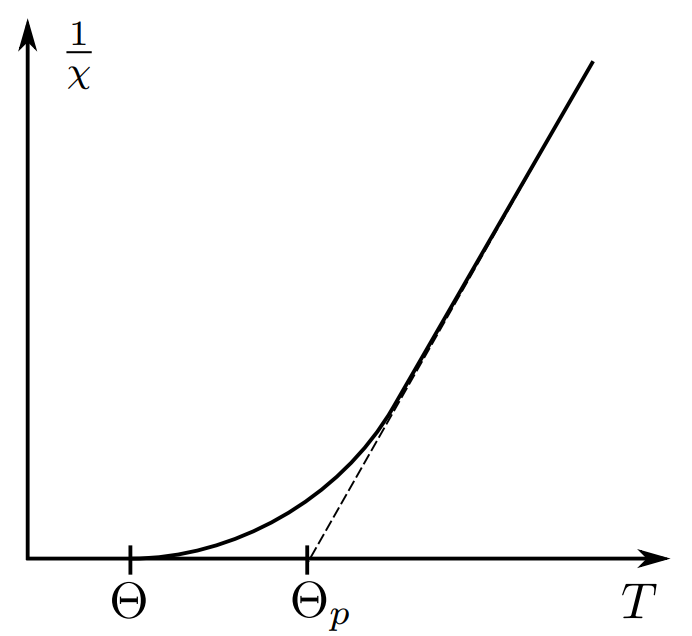
\includegraphics[width=1\textwidth]{3.4.2_1.png}
    \textbf{Рис. 1.} Зависимость обратной величины магнитной восприимчивости от температуры
\end{center}
\end{wrapfigure}

\hfill \break Некоторые ферромагнетики при повышении температуры испытывают фазовый переход в парамагнитное состояние. При малых температурах тепловое движение меньше препятствует магнитным моментам атомов ориентироваться в одном направлении при сколь угодно слабом внешнем поле. Температуру фазового перехода второго рода парамагнетик ($T > \Theta_\text{к}$)-ферромагнетик($T < \Theta_\text{к}$) называют \textit{температурой Кюри} $\Theta_\text{к}$. Температурная зависимость магнитной восприимчивости у ферромагнетиков выше точки Кюри  описывается \textit{законом Кюри-Вейсса}:

\begin{equation}\label{ linkname }
\chi \propto \frac{1}{T-\Theta_{p}},
\end{equation}

\hfill \break где $\Theta_{p}$ $-$ параметр с размерностью температуры, называемый \textit{парамагнитной точкой Кюри}. Величина $\Theta_{p}$ близка к $\Theta_\text{к}$, но не совпадает с ней. Закон Кюри-Вейсса удовлетворительно выполняется вдали от $\Theta_\text{к}$, однако нарушается при приближении к этой точке перехода, где модель среднего поля становится слишком груба. На практике наблюдается зависимость, изображенная на рис. 1.

\section{Экспериментальная установка}
\hfill \break В работе изучается температурная зависимость $\chi (T)$ гадолиния при температурах выше точки Кюри. Выбор материала определяется тем, что его точка Кюри лежит в диапазоне комнатных температур.

\begin{center}
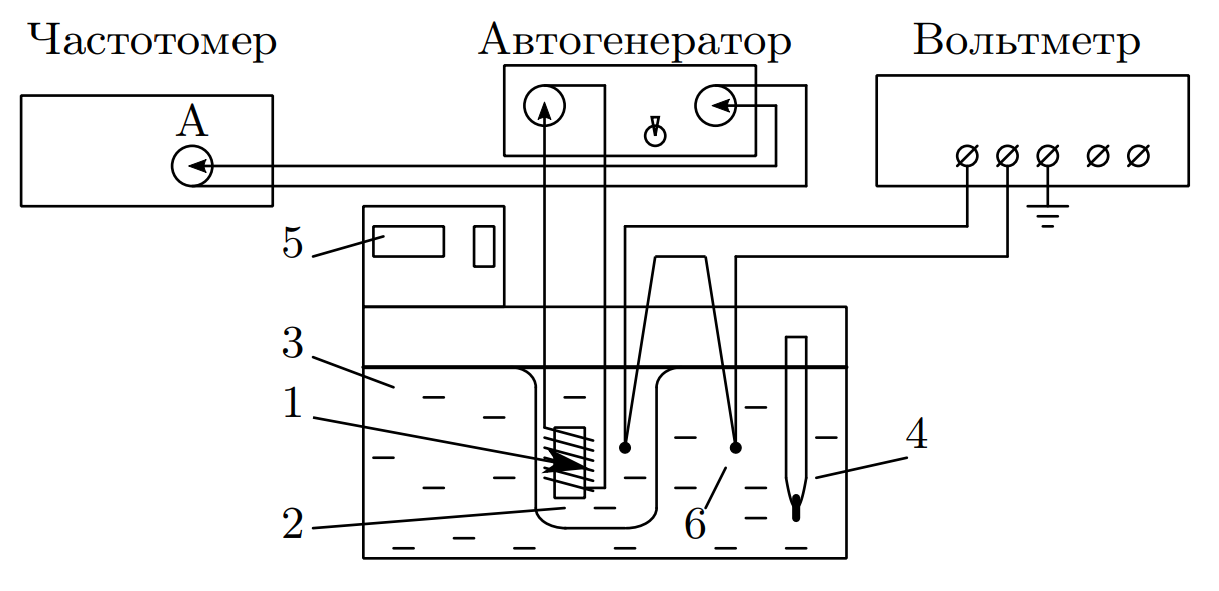
\includegraphics[width=0.75\textwidth]{3.4.2_2.png}\\
\textbf{Рис. 2.}  Схема экспериментальной установки\\ 
\end{center}

\hfill \break Схема установки для проверки закона Кюри-Вейсса показана на рис. 2. Исследуемый ферромагнитный образец расположен внутри пустотелой катушки самоиндукции, которая служит индуктивностью колебательного контура, входящего в состав $LC$-автогенератора (генератора колебаний с хорошим самовозбуждением).

\hfill \break Катушка 1 с образцом помещена в стеклянный сосуд 2, залитый трансформаторным маслом. Масло предохраняет образец от окисления и способствует ухудшению электрического контакта между отдельными частичками образца. Кроме того, оно улучшает тепловой контакт между образцом и термостатной (рабочей) жидкостью 3 в термостате. Ртутный термометр 4 используется для приближенной оценки температуры. Температура образца регулируется с помощью термостата 5.

\hfill \break Коэффициент самоиндукции катушки $L$ пропорционален магнитной проницаемости $\mu$ заполняющей его среды: $L \propto \text{Ф} \propto B \propto \mu$. Тогда разность самоиндукций катушки с образцом $L$ и без него $L_{0}$ будет пропорциональна восприимчивости образца $\chi$:

$$
L-L_{0} \propto \mu - 1 = \chi.
$$

\hfill \break При изменении индуктивности образца меняется период колебаний автогенератора:

\begin{equation}\label{ linkname }
\tau = 2\pi \sqrt{LC},
\end{equation}

\hfill \break где $C$ $-$ емкость контура автогенератора. Аналогичным (8) образом определяется период колебаний в отсутствие образца:

\begin{equation}\label{ linkname }
\tau_{0} = 2\pi \sqrt{L_{0}C}.
\end{equation}

\hfill \break Тогда

$$
L-L_{0} \propto \tau^2-\tau_{0}^2,
$$

\hfill \break то есть, следовательно,

$$
\chi \propto \tau^2 - \tau_{0}^2.
$$

\hfill \break Отсюда следует, что закон Кюри-Вейсса справедлив, если выполнено соотношение

\begin{equation}\label{ linkname }
\frac{1}{\tau^2 - \tau_{0}^2} \propto T - \Theta_{p}.
\end{equation}

\hfill \break Измерения проводятся в интервале температур от 14 до 40 градусов. Температура исследуемого образца всегда несколько отличается от температуры воды в термостате. После того как вода достигла заданной температуры, идет медленный процесс выравнивания температур образца и воды. Разность их температур контролируется с помощью медно-константановой термопары 6, один из спаев которой находится в тепловом контакте с образцом, а другой погружен в воду, и цифрового вольтметра, к которому подключены концы термопары.

\section{Ход работы}

\hfill \break Подготовим приборы к работе и запишем параметры установки: чувствительность термопары $k = 24$ град/мВ; зная допустимую разность температур образца и рабочей жидкости $\Delta T = 0.5^\circ C$ (более точному измерению температур мешают паразитные ЭДС, возникающие в цепи термопары), оценим допустимую ЭДС термопары: 

$$
U_{m} = \frac{\Delta T}{k} = \frac{0.5}{24} \approx 0.021 \text{ мВ}.
$$

\hfill \break Также зафиксируем указанный на установке период колебаний без образца ($\tau_{0} = 6.9092$ мкс) и погрешности приборов: $\sigma_{T} = 0.01^\circC$, $\sigma_{\tau} = 0.01$ мкс, $\sigma_{\Delta U} = 10^{-5}$ В.

\hfill \break Исследуем зависимость периода колебаний $LC$-генератора от температуры образца, отмечая период колебаний $\tau$ по частотомеру, а температуру $T_{o}$ $-$ по показаниям дисплея термостата и цифрового вольтметра. При этом, как уже было отмечено ранее, температура рабочей жидкости и температура образца, как правило, немного различаются, поэтому температуру образца нужно корректировать при помощи следующей формулы:

$$
T_{o} = T + \Delta Uk,
$$

\hfill \break где $T$ $-$ температура, которую отображает дисплей, $\Delta U$ $-$ показание вольтметра в момент измерения периода. Термопара подключена так, что при знаке <<->> на табло вольтметра температура образца ниже температуры рабочей жидкости. Результаты исследования занесем в таблицу 1:

\begin{center}
\begin{tabular}{|c|c|c|c|c|c|c|}\hline
$ n $ & $ T, \text{ } ^\circ C $ & $ \Delta U $, мкВ & $ T_{0}, \text{ } ^\circ C $ & $ \tau $, мкс & $ \tau^2 - \tau_{0}^2 $, $ \text{мкс}^2 $ & $ \frac{1}{\tau^2 - \tau_{0}^2} $, $ \text{мкс}^{-2} $ \\\hline
1 & 14.11 & -0.021 & 13.61 & 7.979 & 15.927 & 0.063 \\\hline
2 & 16.09 & -0.021 & 15.59 & 7.920 & 14.989 & 0.067 \\\hline
3 & 18.08 & -0.024 & 17.50 & 7.827 & 13.525 & 0.074 \\\hline
4 & 20.09 & -0.024 & 19.51 & 7.657 & 10.893 & 0.092 \\\hline
5 & 22.08 & -0.022 & 21.55 & 7.448 & 7.736 & 0.129\\\hline
6 & 24.07 & -0.025 & 23.47 & 7.275 & 5.189 & 0.193 \\\hline
7 & 26.09 & -0.021 & 25.59 & 7.180 & 3.815 & 0.262 \\\hline
8 & 28.06 & -0.026 & 27.44 & 7.140 & 3.243 & 0.308 \\\hline
9 & 30.08 & -0.022 & 29.55 & 7.100 & 2.673 & 0.374 \\\hline
10 & 32.08 & -0.021 & 31.58 & 7.078 & 2.361 & 0.424 \\\hline
11 & 34.07 & -0.022 & 33.54 & 7.067 & 2.205 & 0.453 \\\hline
12 & 36.07 & -0.021 & 35.57 & 7.052 & 1.994 & 0.502 \\\hline
13 & 38.06 & -0.021 & 37.56 & 7.043 & 1.867 & 0.536 \\\hline
14 & 40.05 & -0.021 & 39.55 & 7.035 & 1.754 & 0.570 \\\hline
\end{tabular} \\
\hfill \break \textbf {Таблица 1.} Расчеты и измерения для определения зависимости периода колебаний от температуры образца\\
\end{center}

\hfill \break Теперь рассчитаем погрешности:

$$
\sigma_{T_{0}} = \sqrt{\sigma_{T} + k^2 \sigma_{\Delta U}^2},
$$

\hfill \break но $\sigma_{\Delta U}$ очень мала по сравнению с $\sigma_{T}$, поэтому можно считать, что $\sigma_{T_{0}} \approx \sigma_{T}$.

$$
\sigma_{\frac{1}{\tau^2 - \tau_{0}^2}} = \frac{\partial \left( \frac{1}{\tau^2 - \tau_{0}^2} \right)}{\partial \tau} \sigma_{\tau} = \frac{2\tau \sigma_{\tau}}{\left(\tau^2 - \tau_{0}^2\right)^2}.
$$

\hfill \break Результаты расчета погрешностей занесем в таблицу 2:

\begin{center}
\begin{tabular}{|c|c|c|}\hline
$ n $ & $ \tau $, мкс & $ \sigma_{\frac{1}{\tau^2 - \tau_{0}^2}} $, $\text{мкс}^{-2} $ \\\hline
1 & 7.979 & 0.001 \\\hline
2 & 7.920 & 0.001 \\\hline
3 & 7.827 & 0.001 \\\hline
4 & 7.657 & 0.001 \\\hline
5 & 7.448 & 0.002 \\\hline
6 & 7.275 & 0.005 \\\hline
7 & 7.180 & 0.010 \\\hline
8 & 7.140 & 0.014 \\\hline
9 & 7.100 & 0.020 \\\hline
10 & 7.078 & 0.025 \\\hline
11 & 7.067 & 0.029 \\\hline
12 & 7.052 & 0.035 \\\hline
13 & 7.043 & 0.040 \\\hline
14 & 7.035 & 0.046 \\\hline
\end{tabular} \\
\hfill \break \textbf {Таблица 2.} Погрешности\\
\end{center}

\hfill \break Построим график зависимости вида $f(T) = \frac{1}{\tau^2 - \tau_{0}^2}$ (рис. 3) и экстраполируем полученную кривую к оси абсцисс. Зная соотношение (10) $\frac{1}{\tau^2 - \tau_{0}^2} \propto T - \Theta_{p}$, можно определить, что парамагнитная точка Кюри $\Theta_{p}$ будет лежать на пересечении линейного участка полученной кривой и оси абсцисс, по которой отложена температура образца.

\begin{center}
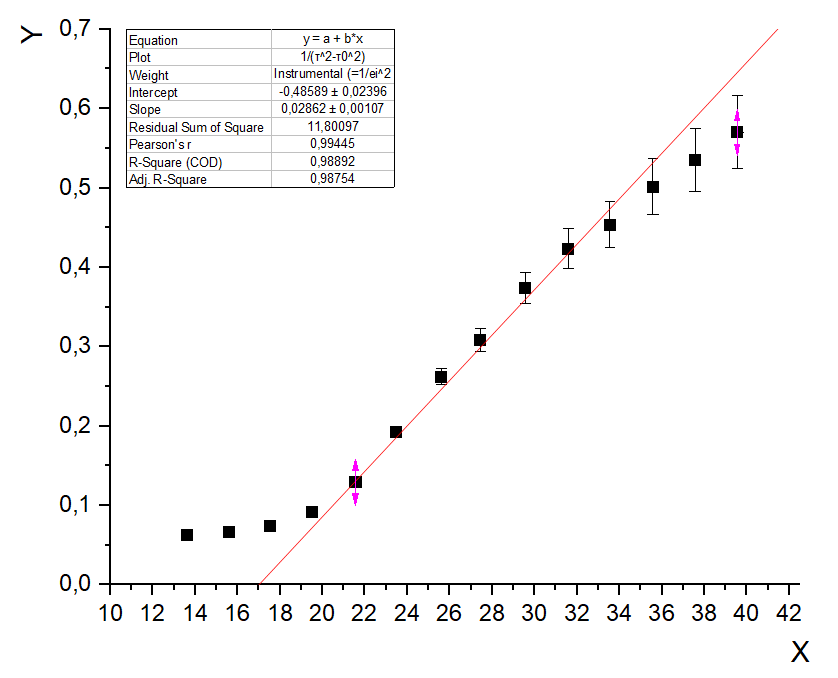
\includegraphics[width=0.85\textwidth]{3.4.2_3.png}\\
\textbf{Рис. 3.} График зависимости $f(T) = \frac{1}{\tau^2 - \tau_{0}^2}$, где $x \equiv T_{o}$ $-$ температура образца, $y \equiv \frac{1}{\tau^2 - \tau_{0}^2}$\\
\end{center}

\hfill \break Линейный участок кривой можно представить в виде $y = a + bx$, значения коэффцицентов $a$ и $b$ и погрешностей их определения занесем в таблицу 3:

\begin{center}
\begin{tabular}{|c|c|c|c|}\hline
$ a $ & $ \sigma_{a} $ & $ b $ & $ \sigma_{b} $ \\\hline
-0.486 & 0.024 & 0.029 & 0.001 \\\hline
\end{tabular} \\
\hfill \break \textbf {Таблица 3.} Коэффициенты аппроксимированной прямой $y = a + bx$\\
\end{center}

\hfill \break Отсюда можно найти парамагнитную точку Кюри для гадолиния: $\Theta_{p} \approx 17.01^\circ C$. Погрешность можно определить по следующей формуле:

$$
\sigma_{\Theta_{p}} = \Theta_{p} \sqrt{\left( \frac{\sigma_{a}}{|a|} \right)^2 + \left( \frac{\sigma_{b}}{b} \right)^2} \approx 1.02^\circ C.
$$

\hfill \break Таким образом, найденная экспериментальным путем парамагнитная точка Кюри для гадолиния: $\Theta_{p} = (17.01 \pm 1.02)^\circ C$. Сравним с теоретическим значением, найденным в интернете, $-$ примерно $17^\circ C$, что совпадает с вычисленным значением в пределах погрешности.

\section{Вывод}
\hfill \break В ходе работы была экспериментально определена парамагнитная точка Кюри для гадолиния, исследован его переход из ферромагнитного в парамагнитное состояние. Полученное значение хорошо совпало с табличным.

\end{document}
